\section{MAXED}\label{MAXED_description}
An introduction about MAXED and the reasons it was developed will go here.

\subsection{Description of the math of detector response unfolding}\label{MAXED_math}
Talk about dual annealing, the maximum entropy method, $\chi^2$ method.

\subsection{Passive Neutron Spectrometer Response}\label{PNS_response}
The Passive Neutron Spectrometer provides similar capabilities to multisphere neutron spectrometers (like Bonner spheres), albeit in a single sphere of material. With the 55 TLDs arranged along the three Cartesian axes, each detector has a different thickness of material separating it from a potential neutron source. This arrangement effects a different response in each of the TLDs, which can be utilized in unfolding techniques.

A typical depth-averaged (I'll have described this in an earlier chapter/section) detector response from the PNS is shown in Figure \ref{example_PNS_dr}.

\begin{figure}[H]
  \centering
  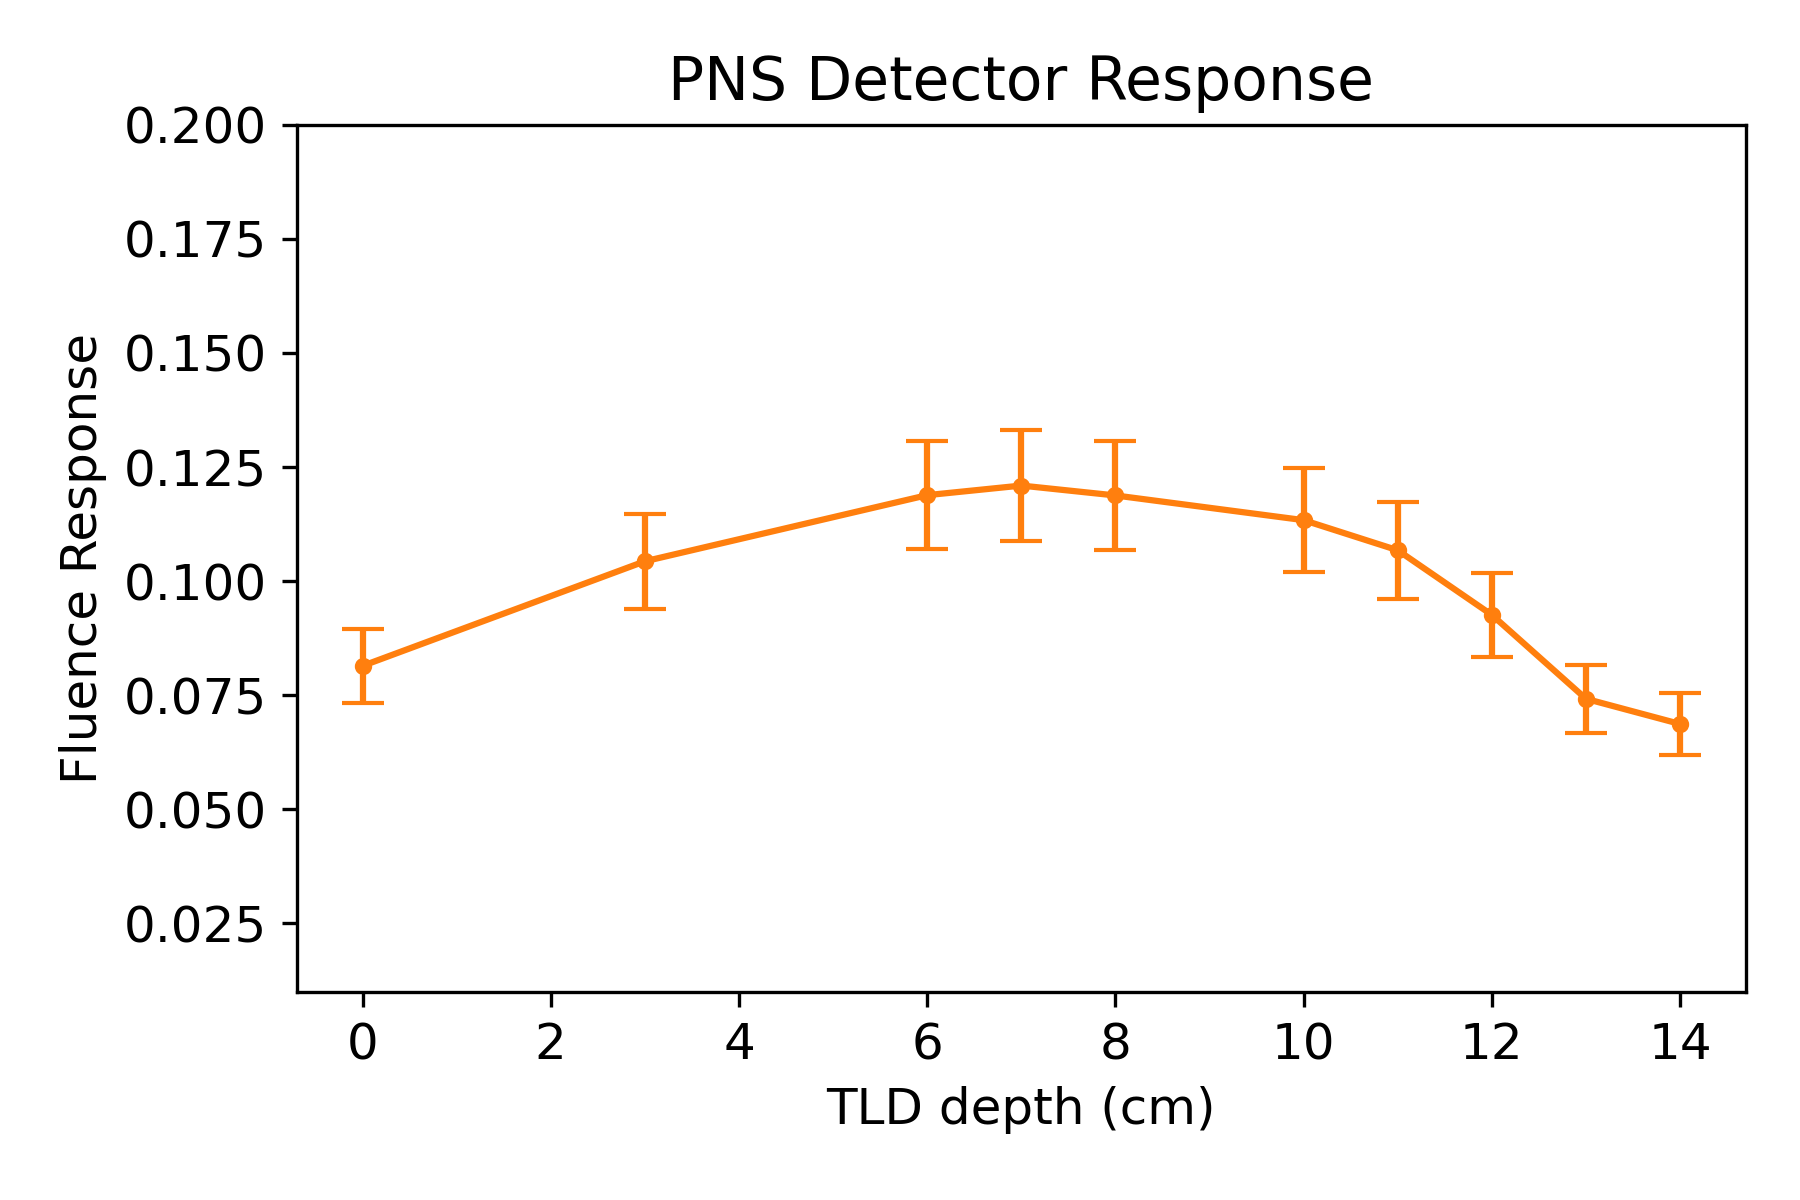
\includegraphics[scale=0.9]{images/Example_PNS_dr.png}
  \caption{A depth-averaged detector response from the PNS in the presence of a Cf-252 neutron source.} \label{example_PNS_dr}
\end{figure}

\subsection{Unfolding the Detector Response}
(The math will be described in Section \ref{MAXED_math})
The detector response from Figure \ref{example_PNS_dr} was used to unfold the neutron spectrum. As mentioned earlier, this detector response was achieved in the presence of a Cf-252 source. Knowing the correct spectrum allows for a good measurement of the accuracy of the algorithm.
The inputs needed for MAXED to unfold the spectrum is a detector response, an initial guess at what the spectrum should be, and, as mentioned in Section \ref{subsec_drm}, a detector response matrix. The following sections will show the accuracy of MAXED when the guess spectrum is varied and showcases the extreme sensitivity to the initial guess.

Because the true spectrum is known, the accuracy of the output of MAXED can be calculated and compared using the modal assurance criterion (MAC). (Put more information about it here) It gives a range (0 1], 1 being an exact match between two sets of data and anything lower is less similar.

\begin{align}\label{eq:MAC}
MAC = \frac{|(Spectrum_{unfolded})^T(Spectrum_{true})|^2}{((Spectrum_{unfolded})^T(Spectrum_{unfolded}))((Spectrum_{true})^T(Spectrum_{true}))} \,.
\end{align}

\subsection*{Using the true spectrum}
An initial point to check for the accuracy of MAXED is by using the true spectrum as the initial guess. The values for this spectrum were taken from the IAEA document Compendium of Neutron Spectra and Detector Responses for Radiation Protection Purposes \cite{iaea_spec}. Barring any other interactions, the MAXED code should get 100\% accuracy on this example, but because the environment surrounding the PNS will reflect neutrons and affect the detector response, there will still be error. The results of this unfolding is shown in \ref{MAXED_result_PlaneDRM_gs100Cf}.
\begin{itemize}
\item DRM: Plane source DRM
\item Guess Spectrum: Cf-252 spectrum
\end{itemize}

\begin{figure}[htb]
  \centering
  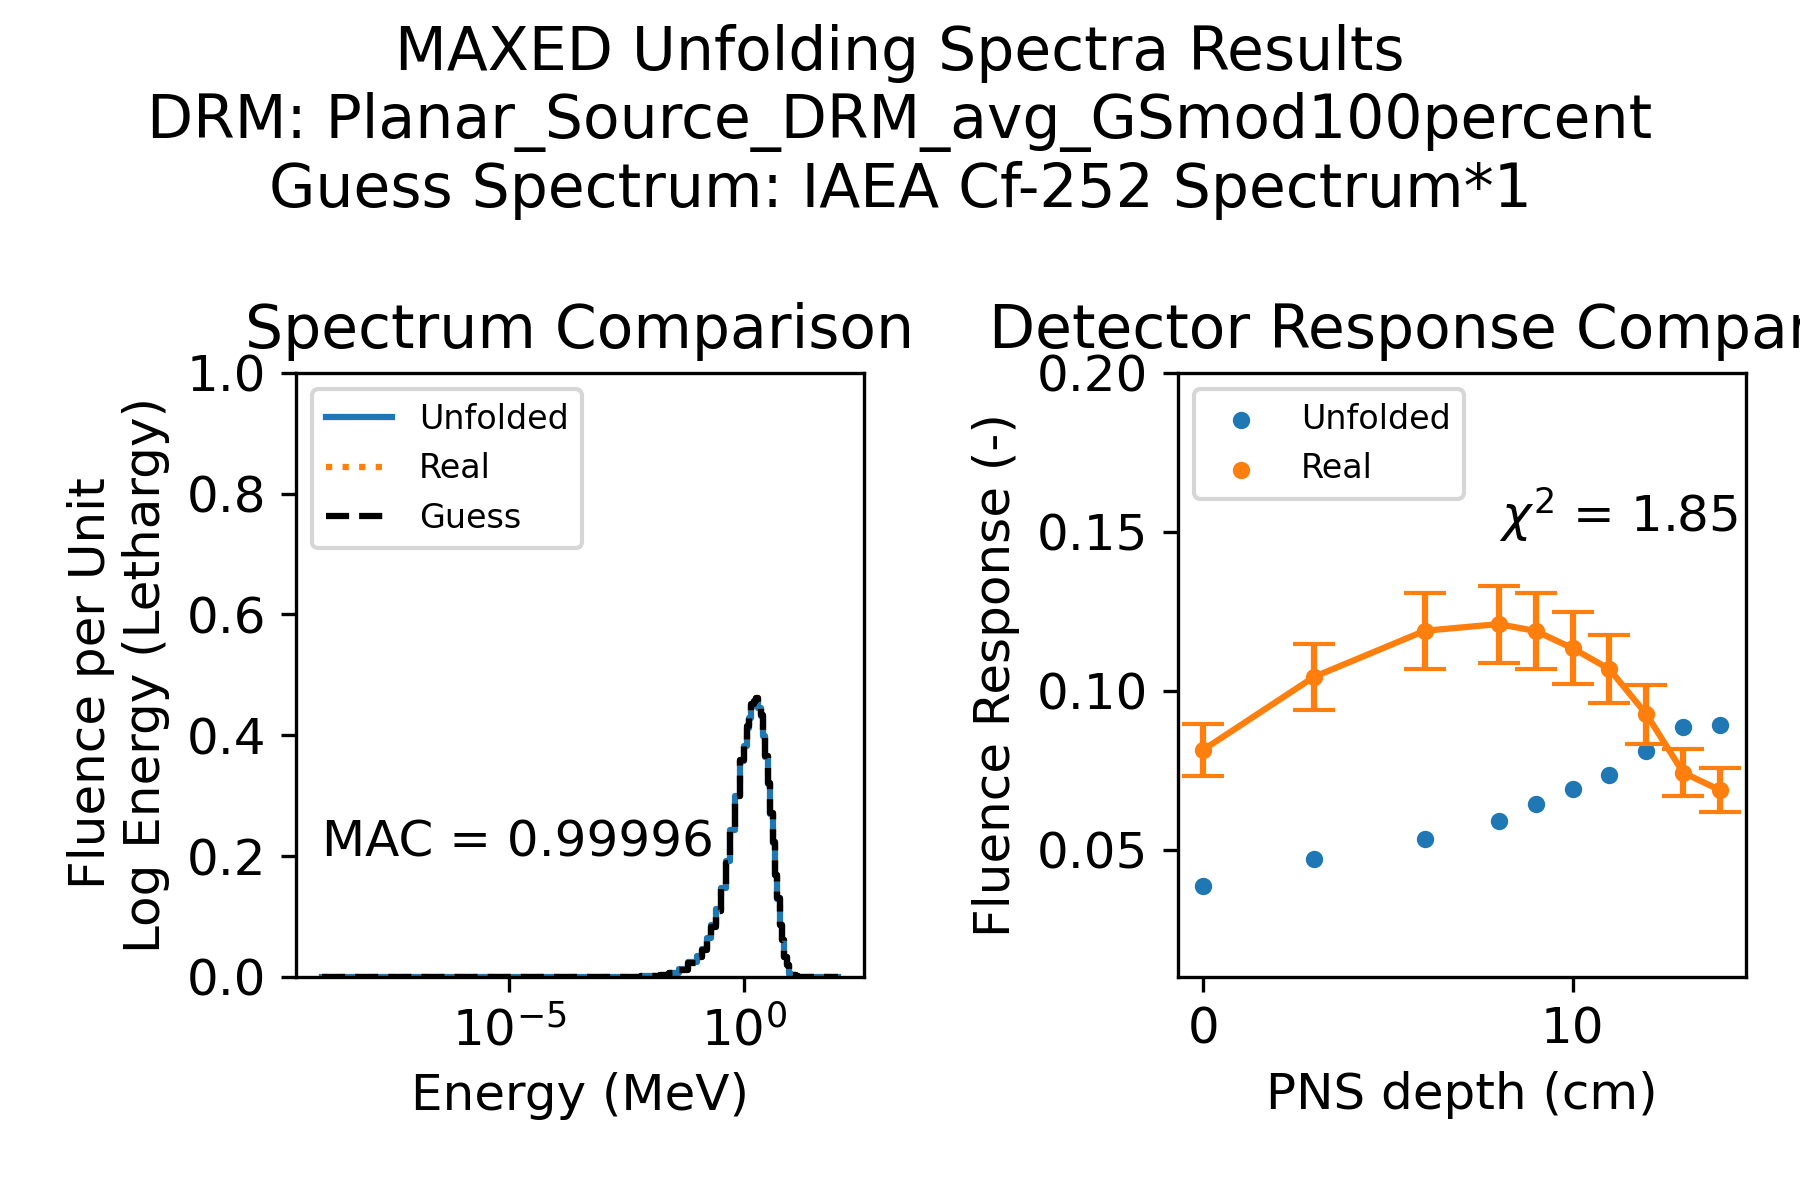
\includegraphics[scale=0.8]{images/Planar_Source_DRM_avg_GSmod100percent_IAEA Cf-252 Spectrum_0.png}
  \caption{The results of the MAXED algorithm using a Cf-252 guess spectrum.} \label{MAXED_result_PlaneDRM_gs100Cf}
\end{figure}

\subsection*{Using the true spectrum with a different DRM}
Following the above example but with a DRM developing using a spherical source surrounding the PNS and directing neutrons inward. Both are very accurate, with MAC numbers very close to 1. Results are in Figure \ref{MAXED_result_sphereDRM_gs100Cf}
\begin{itemize}
\item DRM: Sphere source DRM
\item Guess Spectrum: Cf-252 spectrum
\end{itemize}

\begin{figure}[htb]
  \centering
  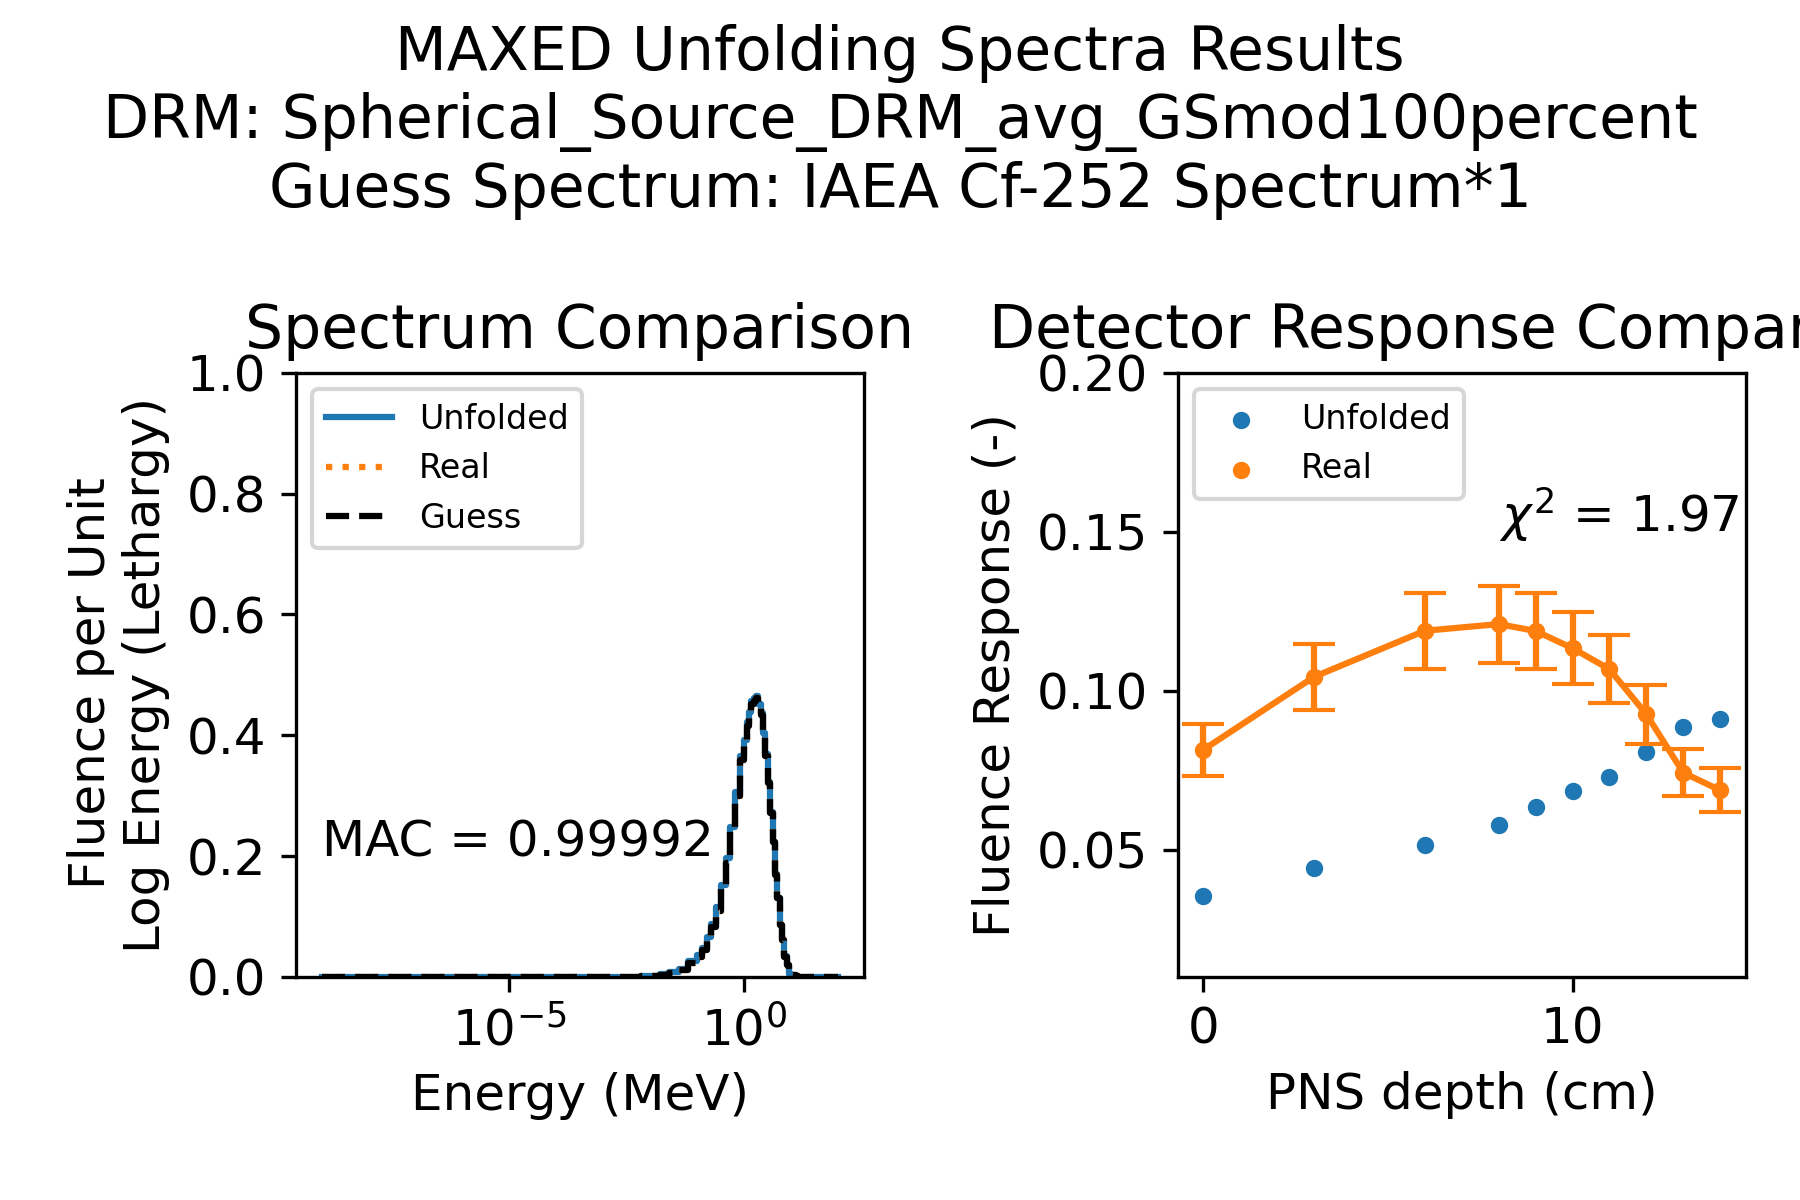
\includegraphics[scale=0.8]{images/Spherical_Source_DRM_avg_GSmod100percent_IAEA Cf-252 Spectrum_0.png}
  \caption{The results of the MAXED algorithm using a Cf-252 guess spectrum.} \label{MAXED_result_sphereDRM_gs100Cf}
\end{figure}

\subsection*{Using the true spectrum multiplied by 0.9}
Running MAXED with the plane-source DRM and using a modified Cf-252 spectrum as the input guess spectrum. The modification was performed by multiplying the spectrum by 0.9. Results are in Figure \ref{MAXED_result_planeDRM_gs90Cf}
\begin{itemize}
\item DRM: Plane source DRM
\item Guess Spectrum: Cf-252 spectrum * 0.9
\end{itemize}

\begin{figure}[htb]
  \centering
  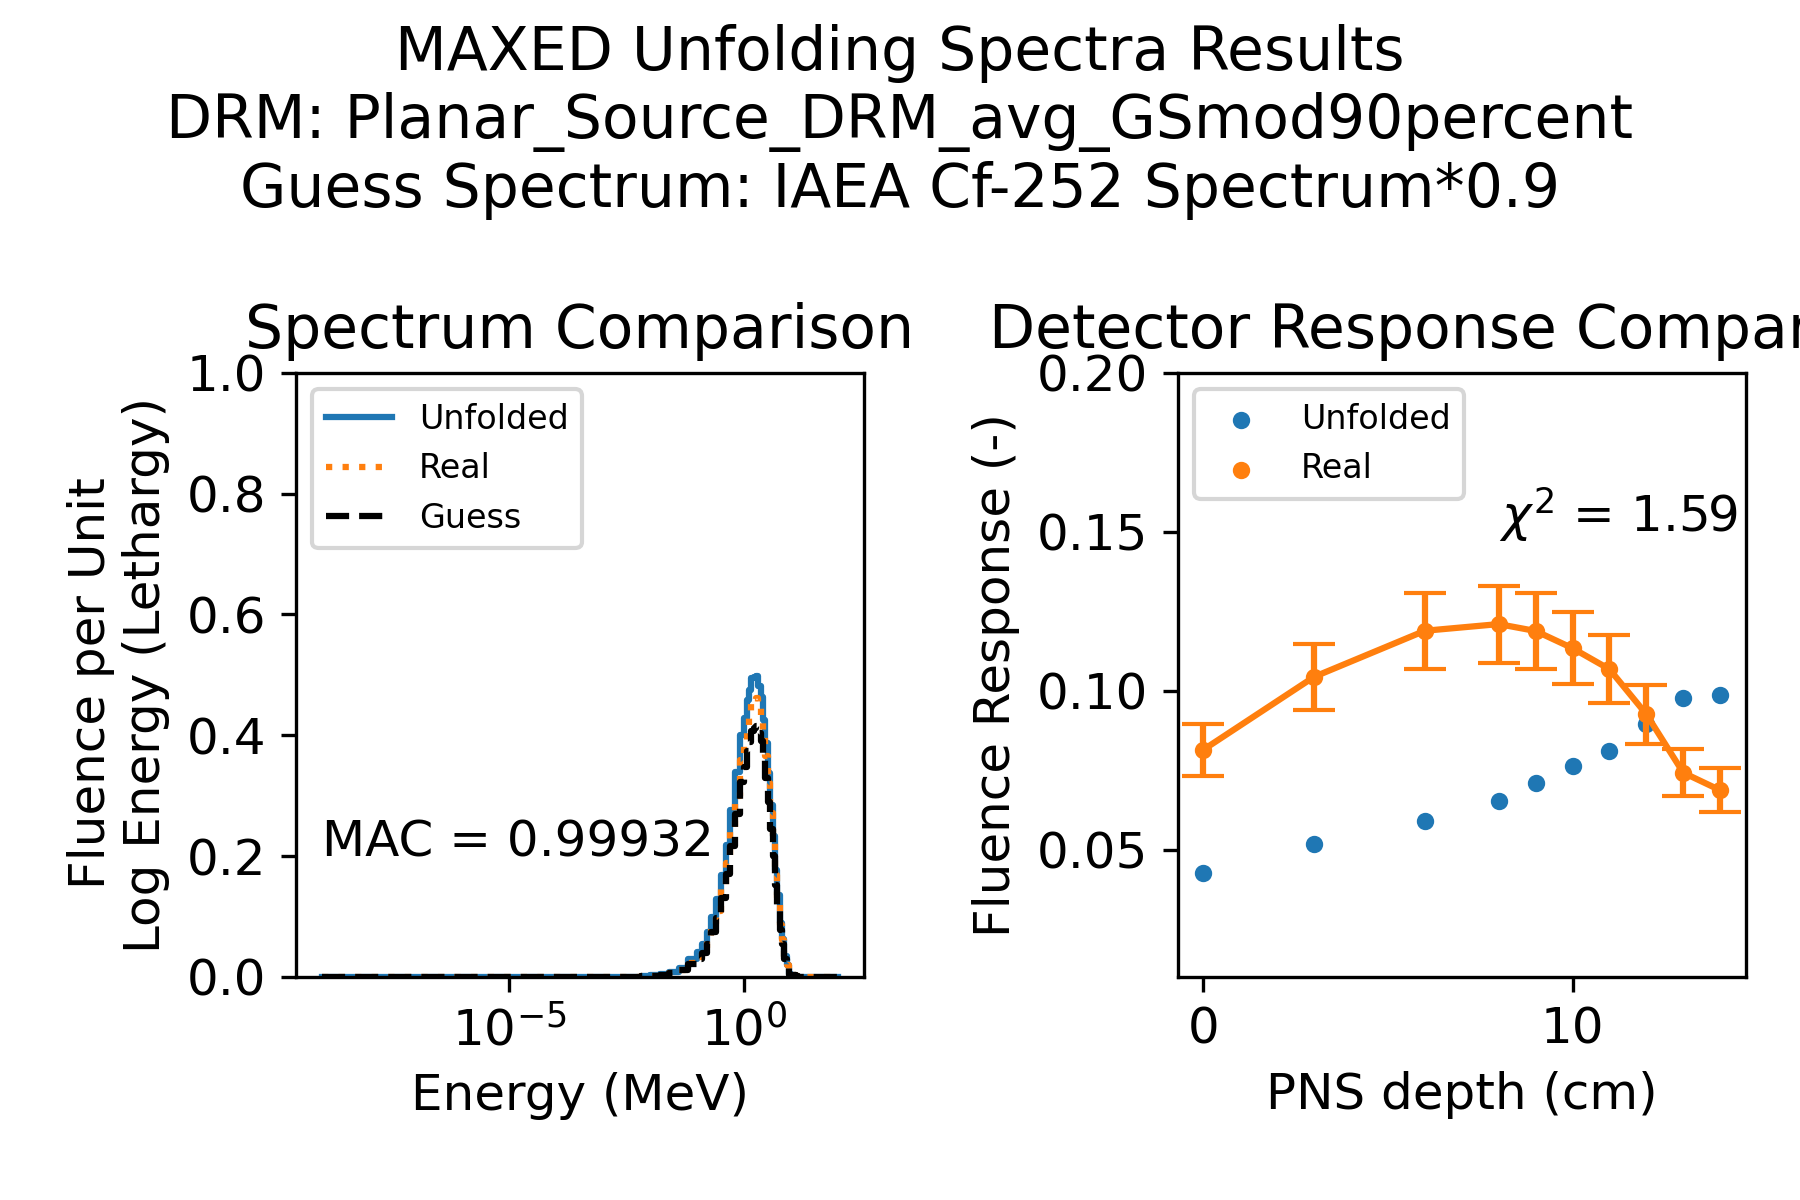
\includegraphics[scale=0.8]{images/Planar_Source_DRM_avg_GSmod90percent_IAEA Cf-252 Spectrum_0.png}
  \caption{The results of the MAXED algorithm using a modified Cf-252 guess spectrum.} \label{MAXED_result_planeDRM_gs90Cf}
\end{figure}

\subsection*{Using the true spectrum multiplied by 0.5}
Running MAXED with the plane-source DRM and using a modified Cf-252 spectrum as the input guess spectrum. The modification was performed by multiplying the spectrum by 0.5. Results are in Figure \ref{MAXED_result_planeDRM_gs50Cf}
\begin{itemize}
\item DRM: Plane source DRM
\item Guess Spectrum: Cf-252 spectrum * 0.5
\end{itemize}

\begin{figure}[htb]
  \centering
  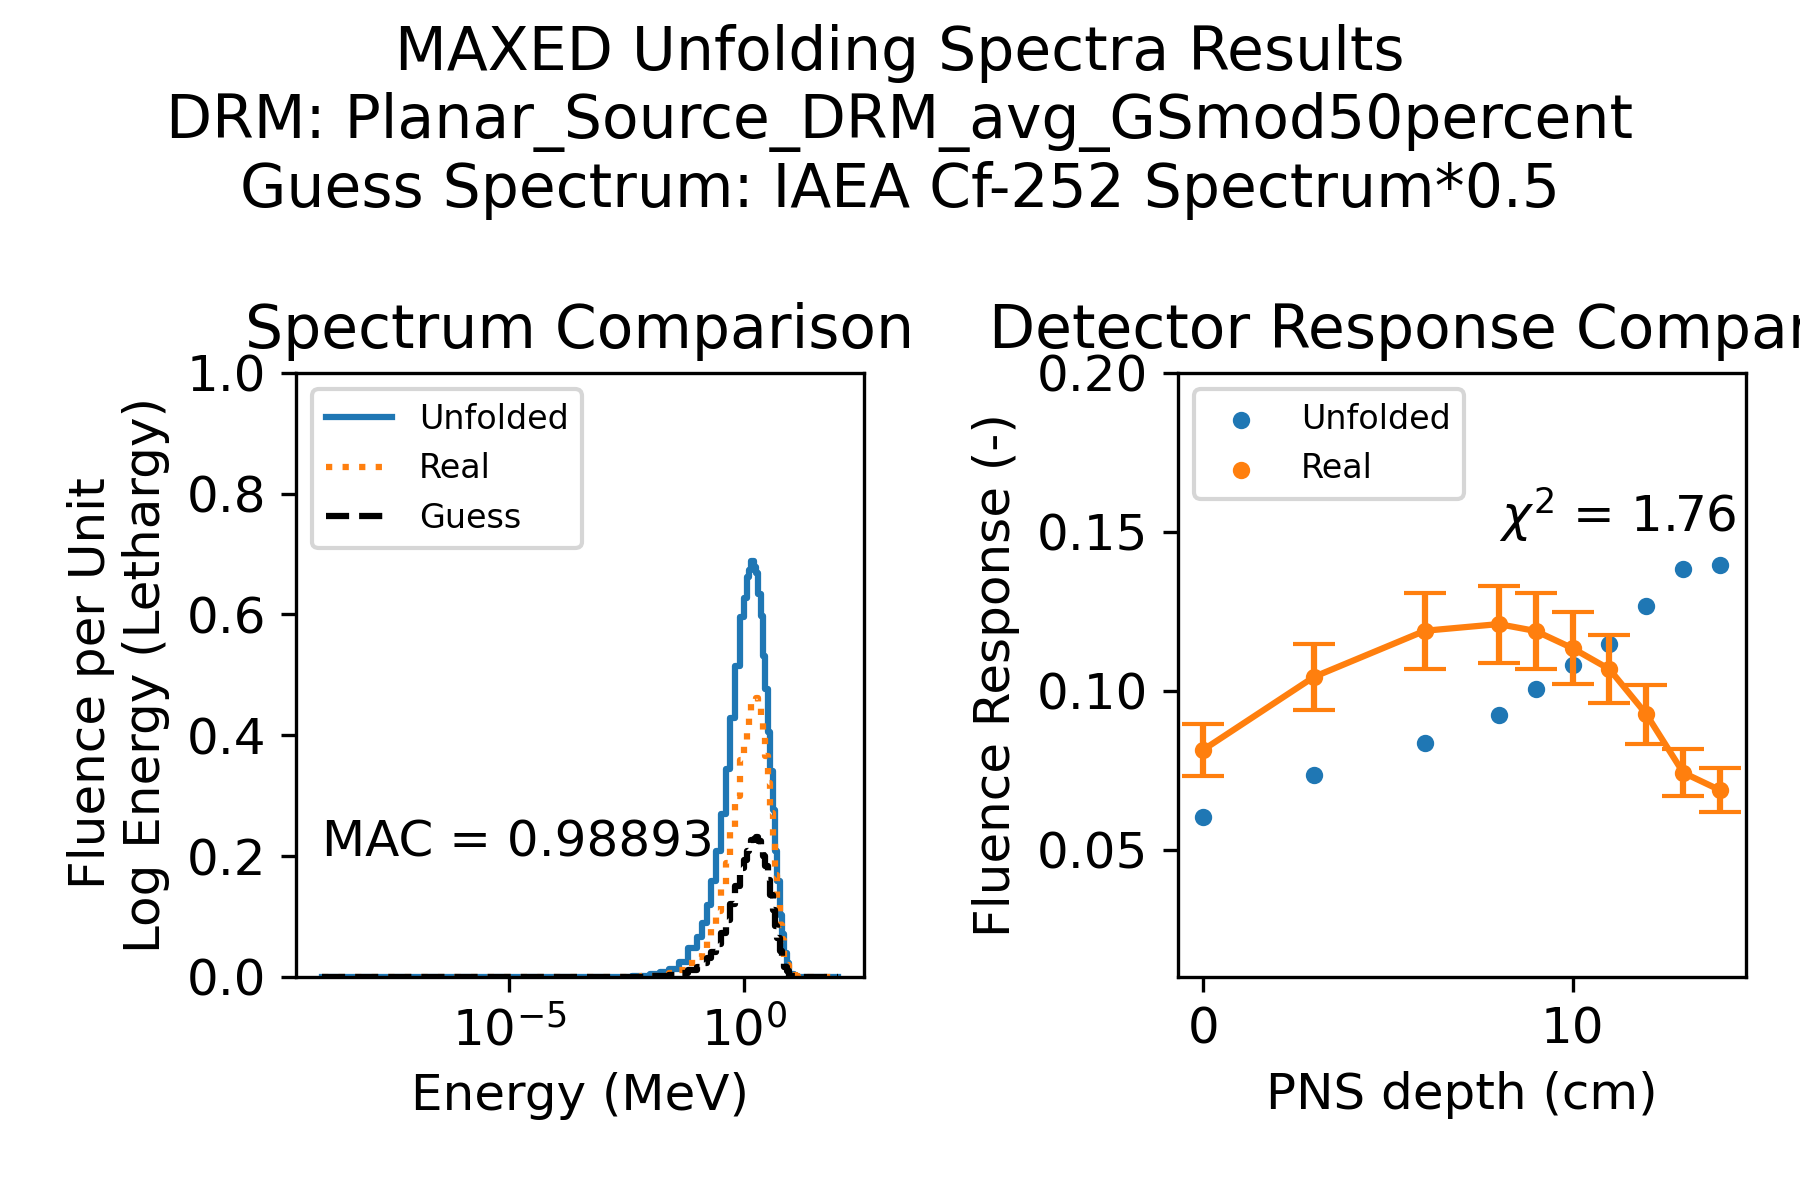
\includegraphics[scale=0.8]{images/Planar_Source_DRM_avg_GSmod50percent_IAEA Cf-252 Spectrum_0.png}
  \caption{The results of the MAXED algorithm using a modified Cf-252 guess spectrum.} \label{MAXED_result_planeDRM_gs50Cf}
\end{figure}

\subsection*{Using a D2O moderated Cf-252 spectrum}
Running MAXED with the plane-source DRM and using a D2O moderated Cf-252 spectrum. Notice that the MAC number is much smaller than 1. Results are in Figure \ref{MAXED_result_planeDRM_gs100D2OmodCf}
\begin{itemize}
\item DRM: Plane source DRM
\item Guess Spectrum: D20 moderated Cf-252 spectrum
\end{itemize}

\begin{figure}[htb]
  \centering
  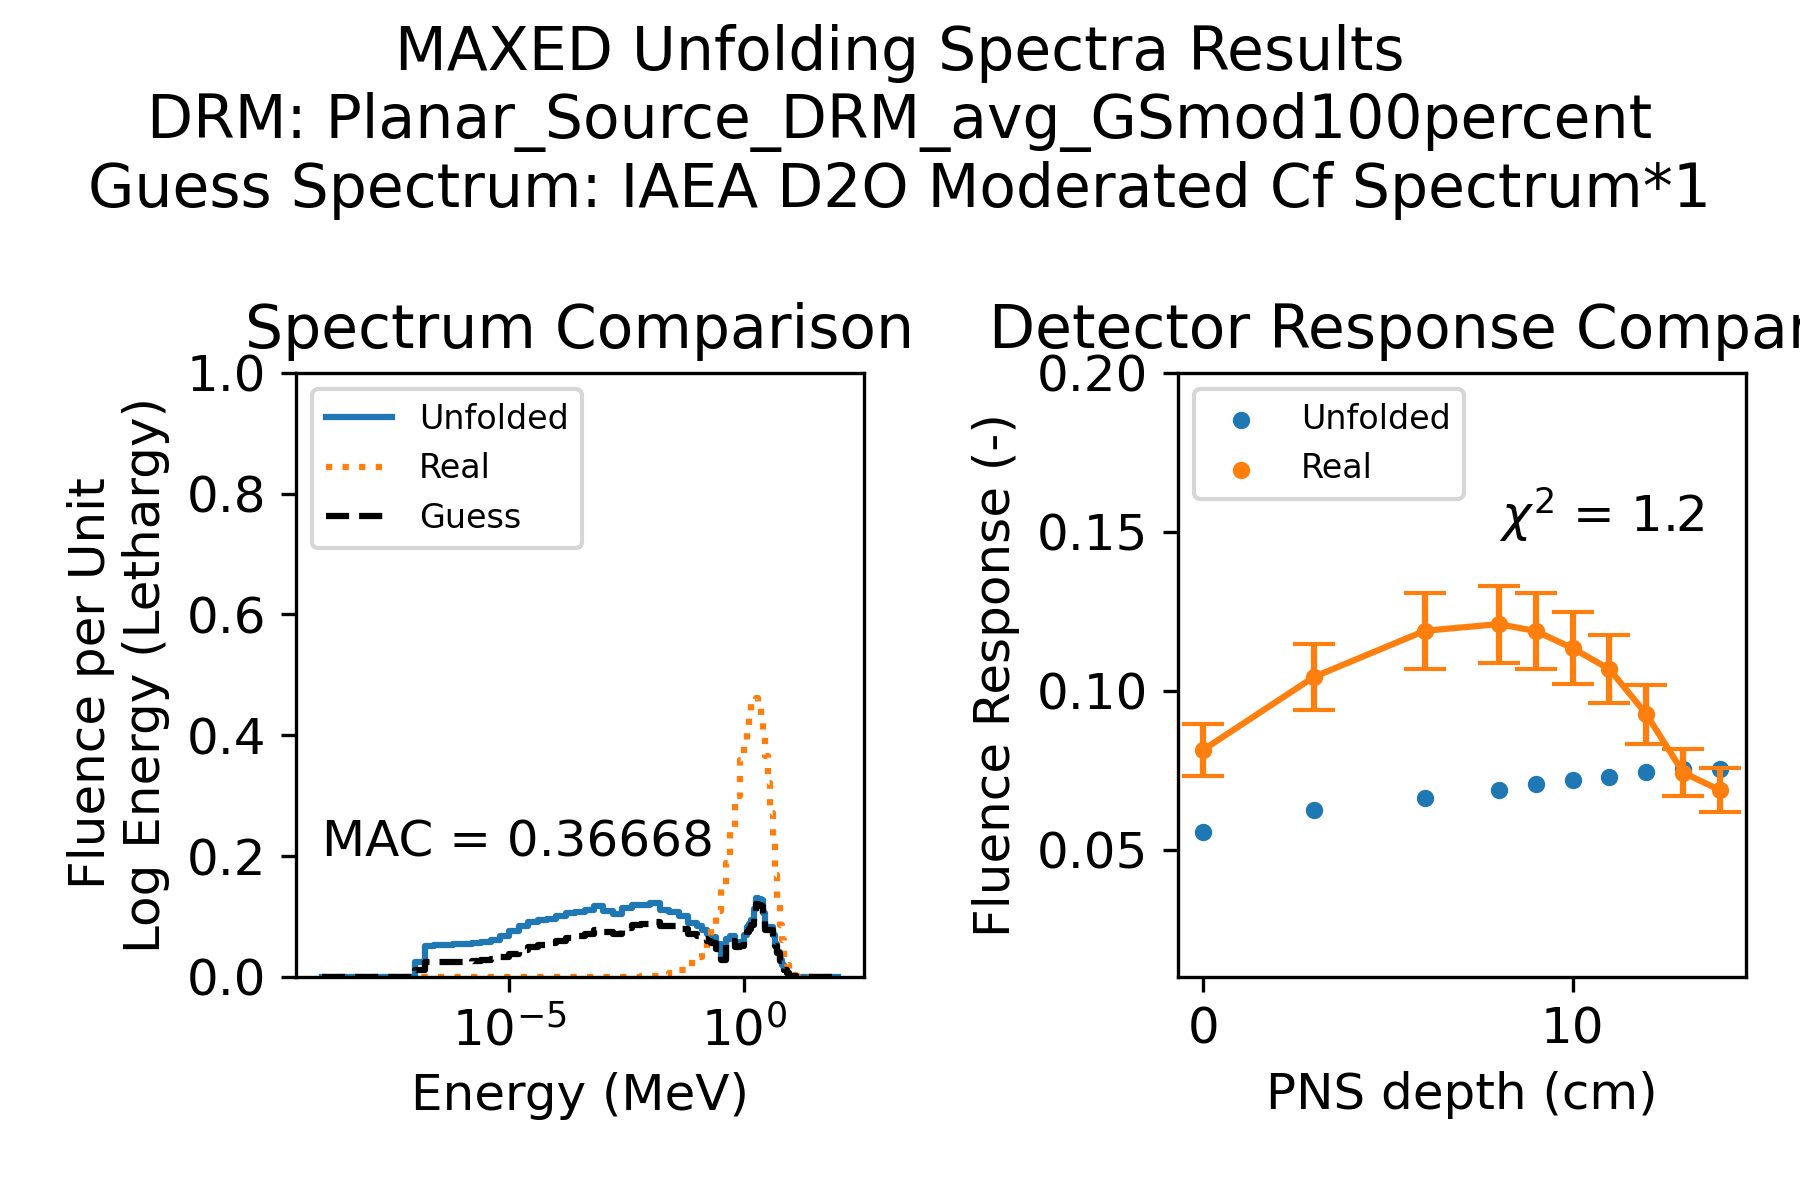
\includegraphics[scale=0.8]{images/Planar_Source_DRM_avg_GSmod100percent_IAEA D2O Moderated Cf Spectrum_0.png}
  \caption{The results of the MAXED algorithm using a D20 moderated Cf-252 guess spectrum.} \label{MAXED_result_planeDRM_gs100D2OmodCf}
\end{figure}

\subsection*{Using a H2O moderated PuBe spectrum}
Running MAXED with the plane-source DRM and using a H2O moderated PuBe spectrum. Notice that the MAC number is much smaller than 1. Results are in Figure \ref{MAXED_result_planeDRM_gs100H2OmodPuBe}
\begin{itemize}
\item DRM: Plane source DRM
\item Guess Spectrum: H2O moderated PuBe spectrum
\end{itemize}

\begin{figure}[htb]
  \centering
  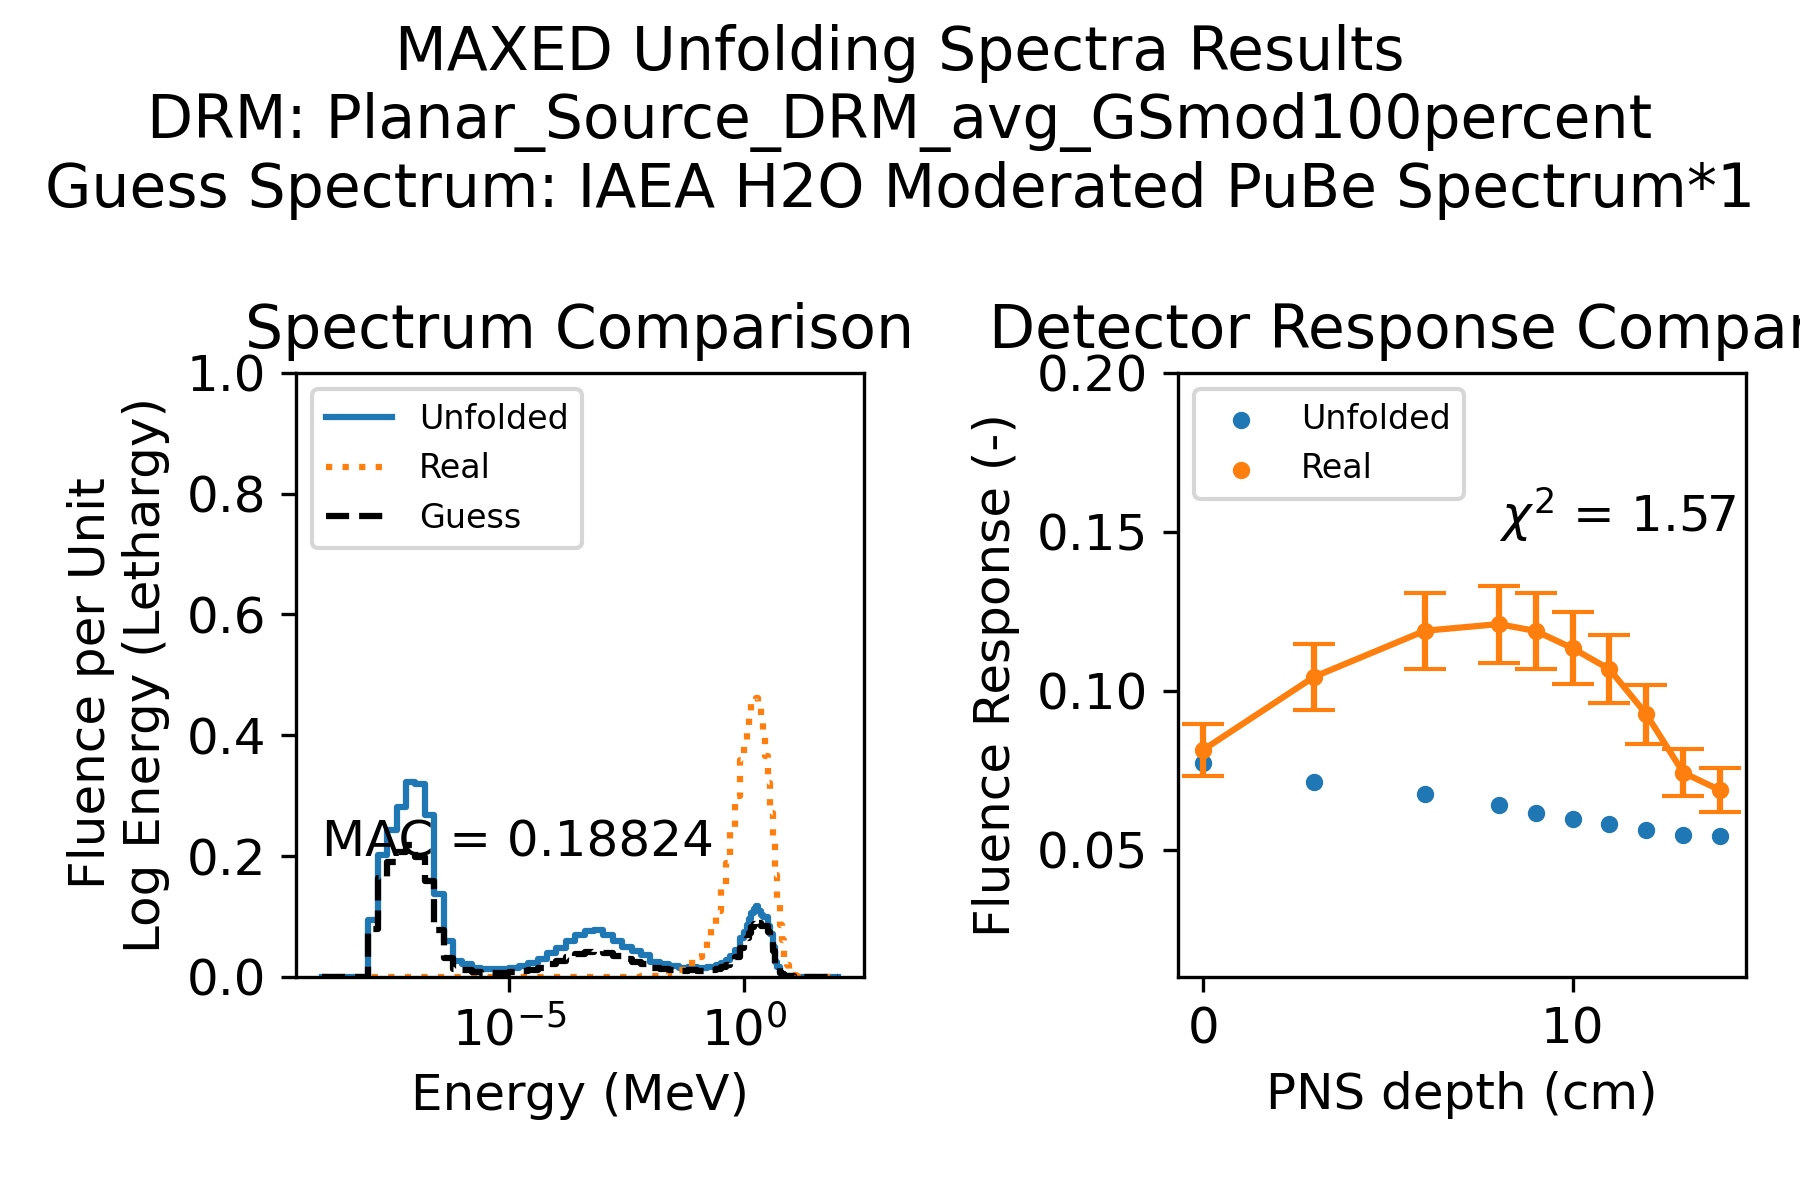
\includegraphics[scale=0.8]{images/Planar_Source_DRM_avg_GSmod100percent_IAEA H2O Moderated PuBe Spectrum_0.png}
  \caption{The results of the MAXED algorithm using a H2O moderated PuBe guess spectrum.} \label{MAXED_result_planeDRM_gs100H2OmodPuBe}
\end{figure}

\subsection*{Using a randomly generated DRM}
Once a different spectrum is used for input, the output of MAXED becomes highly inaccurate. Another test of the robustness is to try using a randomly generated DRM. The results are in Figure \ref{MAXED_result_randomDRM_gs100Cf}. 
\begin{itemize}
\item DRM: Random DRM
\item Guess Spectrum: Cf-252
\end{itemize}

\begin{figure}[htb]
  \centering
  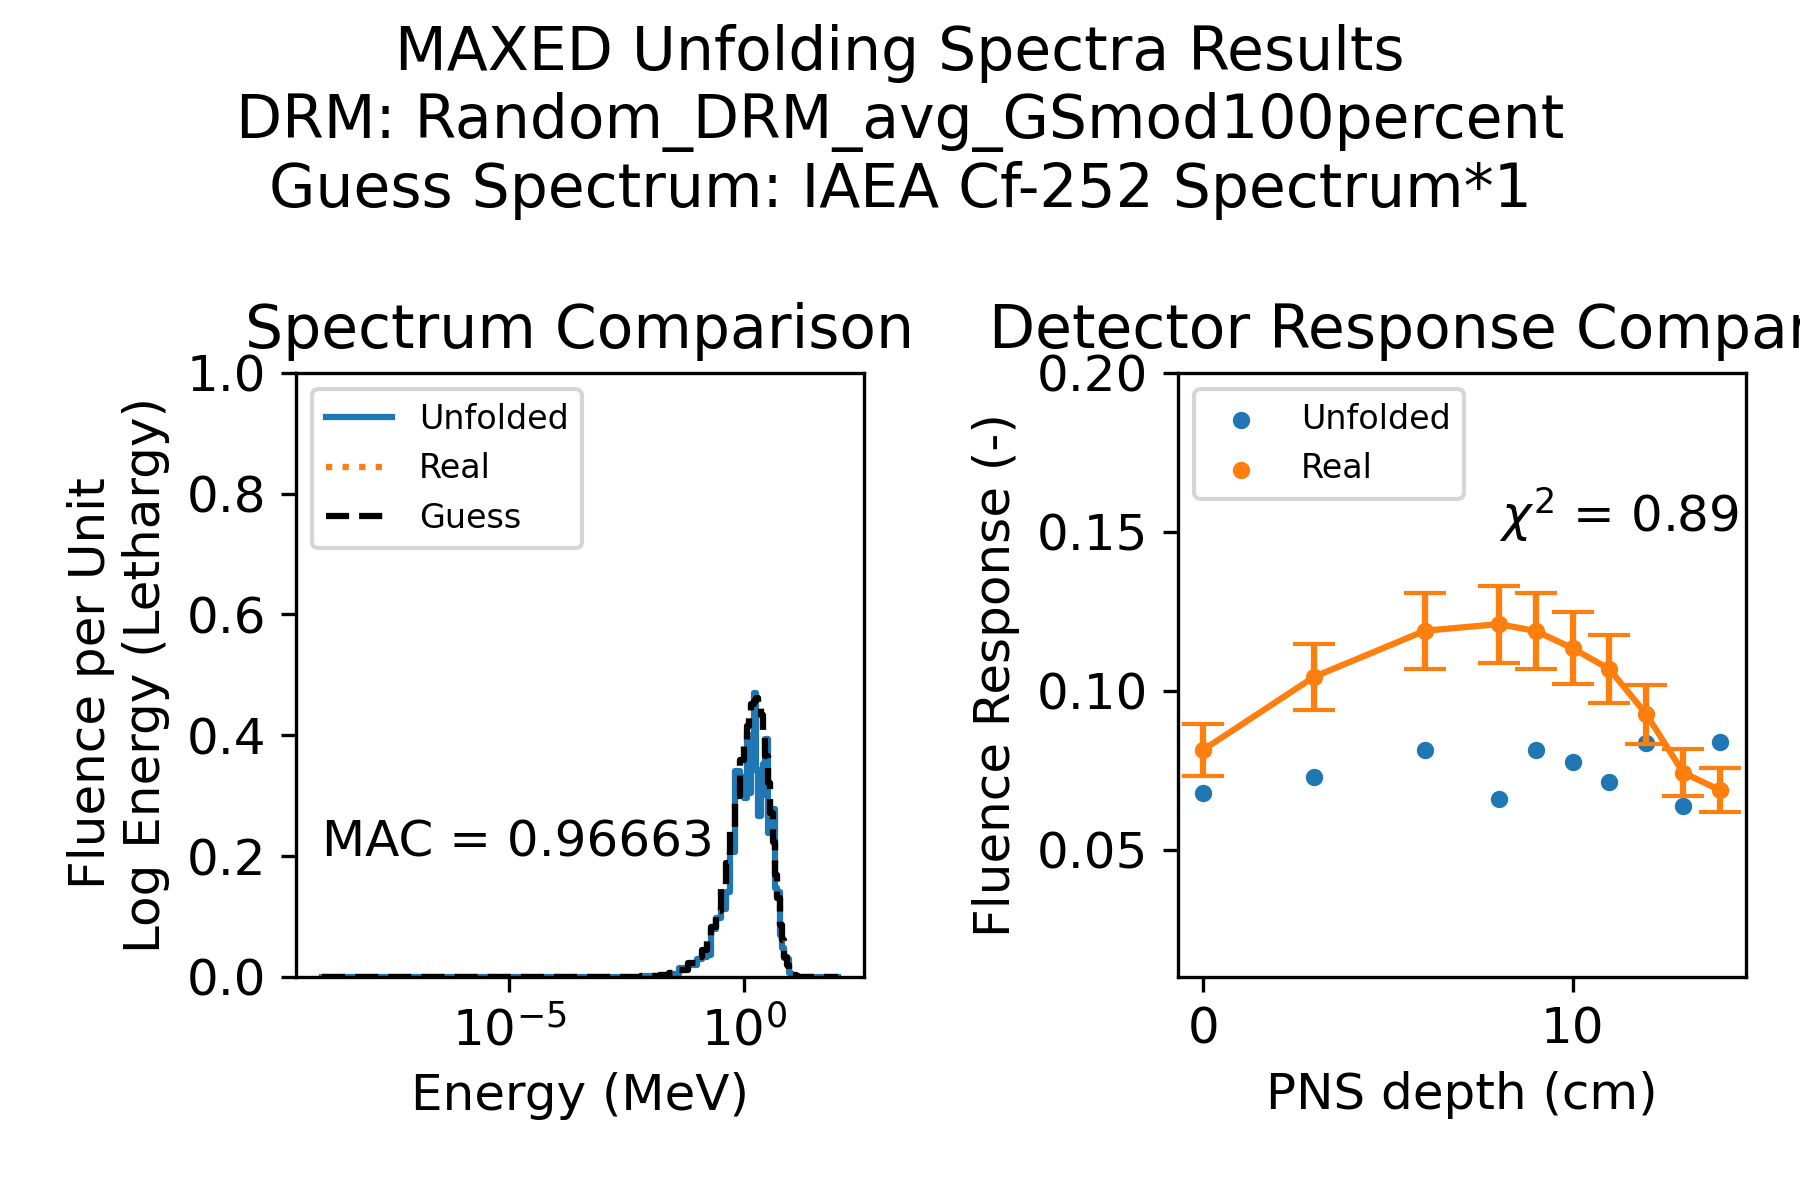
\includegraphics[scale=0.8]{images/Random_DRM_avg_GSmod100percent_IAEA Cf-252 Spectrum_0.png}
  \caption{The results of the MAXED algorithm using a Cf-252 guess spectrum and a randomly generated DRM.} \label{MAXED_result_randomDRM_gs100Cf}
\end{figure}

\subsection*{Using a randomly generated DRM and modified guess spectrum}
The effects of the random DRM are even more visible when the true spectrum is modified like above. In this case, the Cf-252 spectrum is multiplied by 0.5 and the results are in Figure \ref{MAXED_result_randomDRM_gs50Cf}. 
\begin{itemize}
\item DRM: Random DRM
\item Guess Spectrum: Cf-252 * 0.5
\end{itemize}

\begin{figure}[htb]
  \centering
  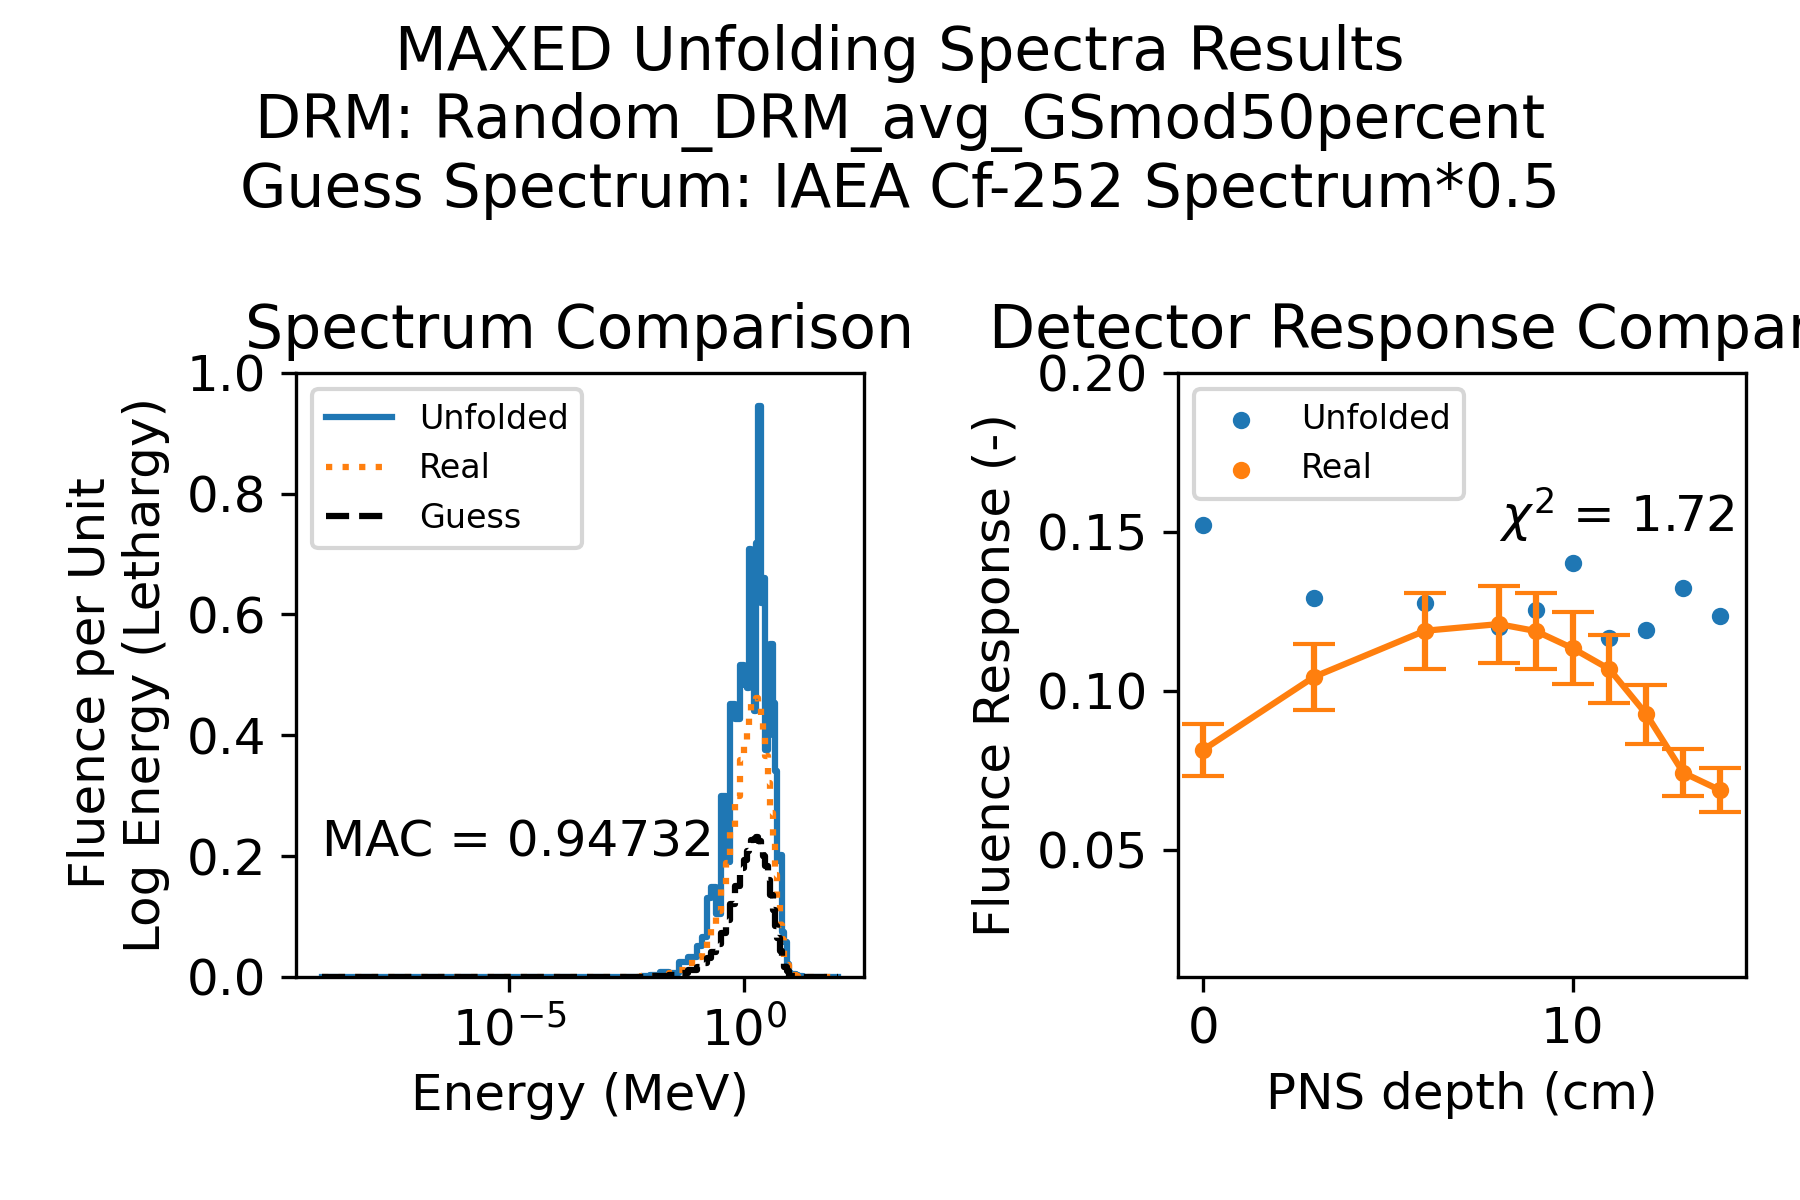
\includegraphics[scale=0.8]{images/Random_DRM_avg_GSmod50percent_IAEA Cf-252 Spectrum_0.png}
  \caption{The results of the MAXED algorithm using a modified Cf-252 guess spectrum and a randomly generated DRM.} \label{MAXED_result_randomDRM_gs50Cf}
\end{figure}

\subsection*{Thoughts on MAXED}
When given very good information, the MAXED algorithm can perform neutron spectrum unfolding. This is highly dependent on the operator who provides the information to the algorithm. As shown in the examples above, the results of MAXED do not depart greatly from the initial guess spectrum. 

At first, it appears that a randomly generated DRM performs well, but I think this is an artifact of the limitations of the MAXED algorithm. I believe that there are a great many local minima and the initial guess makes a very big impact. Additionally, when the guess spectrum is modified like in earlier examples, the effects of the randomness are more pronounced.